% !TeX root = ../main.tex

\chapter{数据驱动的着色器程序性能预测方法}

{\amend 着色器程序是现代图形绘制流水线中决定渲染时间的核心部分之一,本章的引言部分将首先介绍着色器性能预测和优化领域面临的挑战。之后,}本章将提出一种数据驱动的着色器程序性能预测方法,{\amend 该方法利用和程序执行相关、与平台独立的逐指令执行计数,结合平台相关的性能样本进行学习,以构造上下文相关、设备中立的着色器程序性能预测模型。在模型构建过程中,本章将指出若干提升模型表现的设计决策。最后,本章将通过实验和分析,验证本章提出的数据驱动的着色器程序性能预测方法的有效性。}

\section{{\amend 引言}}

\label{sec:ch4_intro}

{\amend 着色器作为嵌入到绘制流水线上的领域专用程序片段,其对 GPU 上实时渲染过程中绘制流水线的执行效率有较大的影响。故而,评估和优化着色器程序对于游戏、VR 交互等实时渲染程序来说至关重要。然而,现有的着色器优化和评估手段存在多种问题:

{\bf 其一},着色器优化在渲染领域一直有一定程度的关注度,但学术界现有的着色器优化工作中所采用的性能评估模型只有{\bf 直接测量}和{\bf 简单线性模型}两种。直接测量是一种平台相关的方法,需要为每个平台重复测量;而简单线性模型则是使用待运行的着色器程序的简单数量特征,其既没有考虑到编译优化、指令和数据相关对于线性启发式中,指令在不同位置执行时间均相等的线性假设的影响,也没有考虑到不同设备的上拥有不同的指令时间的影响。表 \ref{table:shader_optim_work_costs} 给出了现有着色器优化工作中采用的性能评估模型的整理。
}

\begin{table}[h]
    \centering
    \caption{学术界现有的着色器优化工作中所采用的性能评估模型一览}
    \label{table:shader_optim_work_costs}
    \begin{tabular}{l|l|cc}
    \toprule
    \multirow{2}{*}{工作}             & \multirow{2}{*}{发表时间} & \multicolumn{2}{c}{方法} \\
                                    &                     & 直接测量       & 简单线性模型      \\
    \midrule
    \citet{10.1145/2070781.2024186} & 2011                & √          &           \\
    \citet{10.1145/2661229.2661276} & 2014                & √          &           \\
    \citet{10.1145/2816795.2818104} & 2015                &            & √         \\
    \citet{10.1111/cgf.13482}       & 2018                &            & √         \\
    \citet{10.1145/3528233.3530722} & 2022                &            & √         \\
    \bottomrule
    \end{tabular}
\end{table}

{\amend {\bf 其二},计算机体系结构研究领域中,存在一些图形系统的系统建模工作,但这些工作均采用分析模型,且大多不支持着色器程序的模拟。这其中的典型代表为 Emerald \cite{10.1145/3307650.3322221},其利用体系结构模拟的方法实现了一类 TBR(Tile-based Rendering)架构的 GPU SoC 模拟。然而,该工作拥有分析模型的固有缺陷。首先,因为其模拟运行的本质,在其上进行模拟运行并评价性能是相当缓慢的。其次,其运行需要参数的精确对齐,否则预测精度将会受到极大的影响。故而,利用该类方法的思路进行性能预测的成本是相当高昂的。

{\bf 其三},工业界现有的图形优化工具,其可以给出绘制流水线的评估和优化提示,但其采用的预测方法是设备相关、厂商锁定的,且必须在原设备上进行使用和优化。譬如,NVIDIA 公司的 NSight \cite{NSightGraphics} 性能工具就提供了截帧和绘制操作重放、流水线瓶颈分析等功能,但其相关信息均是基于在设备上重放时从 GPU 中读取的性能计数器实现,故而需要相关设备的存在,且只适用于本身测试的设备,对于其它厂商的设备仍然需要不同的软件和方法。

针对上面的问题,本章提出了数据驱动的着色器性能预测方法。该方法的主要优势为如下两个方面:

{\bf 其一},将平台信息融入了着色器代价模型中,并考虑了指令间的上下文联系。学术界现有的着色器优化工作的性能模型主要着眼于给出着色器之间的相对性能顺序,故而采用了平台无关的估计方法。然而,第 \ref{sec:challenge_set_construction} 节的挑战数据集构建与第 \ref{sec:evaluation_challeng_shader} 节的挑战数据集评估和分析表明,着色器之间的相对性能顺序也可能随平台的不同而发生变化。本章提出的方法通过数据驱动的方式,使用各个平台上标注了性能信息的着色器样本进行学习,从而将平台本身的因素融入了着色器代价模型中。同时,通过利用 Transformer 进行序列学习的能力,模型可以学习指令和某次执行作为整体,共同作用得到的时间,而非孤立的认为每条指令的执行时间相同。这样一来,编译变换、延迟隐藏等带来的指令时间与其上下文之间的相关性就得到了考虑。

{\bf 其二},方法本身为平台独立的,其预测过程也不额外需要对待预测平台的访问。相对于体系结构中的图形建模工作来说,本章提出的方法属于数据驱动的方法,且设计过程中的重要目标为不使用平台独占的信息,故而本方法所需要的数据可以在多个平台上以统一的方式进行收集,以解决设备相关和厂商锁定的问题。同时,为了刻画待测试程序的运行时特征,许多工业界的优化方法都依赖模拟器或真实设备运行的结果,而本方法通过采用可以以平台无关的方式得到的指令计数信息来给出程序的运行时信息。
}

\section{{\amend 问题描述和设计思路}}

\label{sec:design_decisions}

{\amend 本章提出的方法旨在用数据驱动的方法解决着色器性能的预测问题。着色器性能预测问题,即给定绘制流水线中的着色器程序,及其相应的运行时输入,预测在某个特定 GPU 平台上的绘制流水线运行时间的问题。作为数据驱动方法,其基本范式为收集该平台上大量的、标注有着色器性能信息的性能样本,利用这些性能样本直接进行目标平台性能特征的学习,再使用训练好的模型预测未知的着色器在该平台上的性能。

从抽象意义上来说,着色器可以抽象为一系列算数逻辑运算和控制流命令的合集。为了捕捉命令之间的相关性,使用序列学习领域的“标准做法”之一的 Transformer 是比较自然的。然而,本章在前期实验中发现,虽然 Transformer 在程序理解方面已经有诸多成功实践,{\bf 但直接利用着色器程序本身,而不加入额外的、和控制流相关的辅助信息,对于预测着色器程序性能的任务来说是困难的}。本章第 \ref{sec:ablation_trace} 节的消融实验即展示了这种情况。从理论分析也可以得到,}尽管着色器本身是一种领域专用语言,但在现代硬件上执行的着色器可以包含动态的循环和分支指令,从而使着色器程序语言在理论上即具有图灵完备性。在图灵完备计算模型内,只基于程序的输入和程序本身来预测其运行时间在理论上的难度等价于求解不可解的停机问题\cite{10.1112/plms/s2-42.1.230}。{\amend 故而,需要设计和程序执行相关的信息送入模型,同时保证其预测时平台独立的性质。}

{\amend 和 CPU 上运行的程序类似,着色器程序也拥有分支和循环等结构,则根据输入的不同,着色器程序执行的总操作可能有所变化。故而,本章选择使用指令计数作为和每次执行相关的额外信息,作为提供给预测模型的辅助输入进行预测工作。这其中,又面临如下几个设计问题:

{\bf 其一,}指令如何规范化表示。着色器程序多以 GLSL、HLSL 或 Slang 等高级着色器程序语言写就,而此类高级程序语言通常具有复杂的指令和控制流表示方式,其“指令”距各种 GPU 上实际执行的指令有较远的距离。\citet{10.1145/3528233.3530722}的着色器优化工作 ShaderTransformer 即试图使用 GLSL 结合着色器的几何输入直接学习着色器质量。其直接使用 GLSL 的设计则限制了其处理的着色器运行时的复杂程度。

从编译器的设计中可知,编译器在编译时通常会将输入的源程序转换为中间表示指令,其可操作性较高级语言描述的指令操作来说粒度更细,便于编辑。图形驱动程序构成的图形栈,其经过十数年的迭代发展,已经创造出了多种开源的中间表示,如 Mesa3D 项目维护的 TGSI\cite{TGSI},NIR\cite{NIR},LLVM 项目维护的 LLVM IR\cite{LLVMIR},Khronos Group 维护的 SPIR-V\cite{SPIRV}等。这其中,SPIR-V 拥有良好的平台无关特性,Vulkan 的官方支持,以及稳定的 ABI 设计,故而本章选择将 GLSL 首先转换为 SPIR-V 指令,以进行规范化表示。

{\bf 其二,}如何进行指令计数跟踪。指令计数跟踪的目的是在规范化表示的指令层次下,给出给定输入下着色器中各个指令的具体执行情况。一种可能的路线是构造一个 SPIR-V 模拟器,将待预测的着色器程序的 SPIR-V 表示和输入信息送入该模拟器,通过模拟执行得到结果。Talvos \cite{Talvos}即是这样的一种模拟器。然而,SPIR-V 定义有数百条指令,且利用 CPU 执行着色器程序需要逐线程模拟着色器程序的每次调用,而不能利用 GPU 本身良好的并行执行能力,进而对指令计数跟踪的效率带来负面的影响。与之相反,本章构造的指令跟踪计数方法,其采用在着色器程序的每个基本块前编排单独的原子增计数指令,以实现在 GPU 执行的指令计数跟踪。

{\bf 其三,}如何设计预测模型。本章提出的预测模型,其骨干基于 Transformer 网络。然而,如果按通常的理解,直接在此任务中设置应用如 BERT 等的网络结构会遇到两个挑战。第一,被第 \ref{sec:ablation_trace} 节消融实验证明重要的指令计数跟踪信息,如何嵌入到网络的输入中。第二,网络预测输出的时间信息如何进行归一化。本章进一步通过两个对比和消融实验证明了所述设计的合理性。

}

\section{{\amend 方法实现}}

\begin{figure}[h]
  \centering
  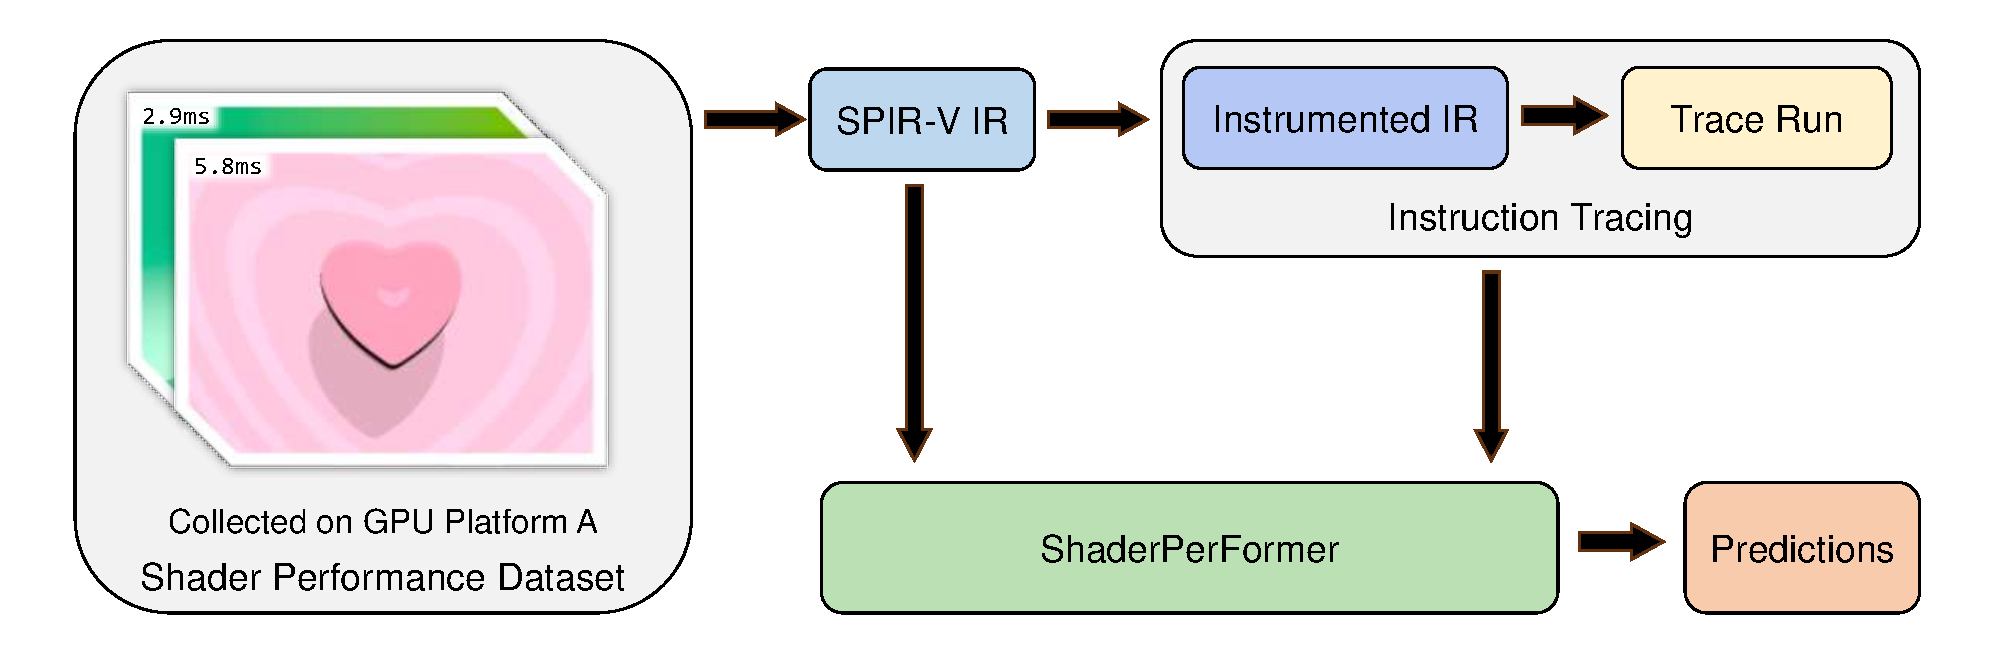
\includegraphics[width=1\linewidth]{figures/OverviewNewNewNew.pdf}
  \caption{本章提出的方法总览}
  % \note{注:图中 GPU 平台 A 是待建模的 GPU 平台,本文提出的模型使用 GPU 平台 A 上收集到的性能数据进行训练。}
  \label{fig:pipeline_overview}
\end{figure}

如图 \ref{fig:pipeline_overview} 所示,本{\amend 章}提出的方法构建了一个针对特定 GPU 平台的着色器性能预测模型。{\amend 该模型利用第 \ref{sec:perf_data_set_chap} 章中构建的着色器性能数据集,首先将着色器程序源码编译为 SPIR-V 指令,然后通过指令计数跟踪过程来获得着色器在给定输入下的执行信息,最后再送入着色器性能预测模型来得到着色器性能在给定平台上的预测结果。}

{\amend SPIR-V 指令的翻译}通过业界的标准着色器编译器 glslang \cite{glslang} 实现,{\amend 其输出为着色器的 SPIR-V 指令流。对于图 \ref{fig:pipeline_overview} 中右上部分的着色器指令跟踪阶段,其输入是着色器程序的 SPIR-V 指令流和给定的着色器运行输入,输出为着色器中每个 SPIR-V 指令在给定的输入下的执行次数。图 \ref{fig:pipeline_overview} 的黄色部分则是利用指令计数信息和着色器的 SPIR-V 表示,进行给定平台下预测着色器进行一次绘制的耗时的预测模型。该模型简称为 ShaderPerFormer。}

{\amend 每个平台需要单独的预测模型。在训练阶段,模型在着色器性能数据集上进行训练,以测量得到的性能真实值作为训练的目标,以梯度下降的方式进行训练。在推理阶段,给出着色器的源码,经过编译、同输入一起进行指令计数跟踪后,将指令计数和 SPIR-V 指令序列送入训练好的网络,即可预测在该平台的性能。指令计数跟踪阶段是平台无关的,其不依赖待测平台,而可以在其它拥有 GPU 的平台上进行,以保证平台独立。}

\subsection{指令计数跟踪}

{\amend 指令计数跟踪阶段的目标是获得着色器转换成的 SPIR-V 指令在给定输入下,程序各指令的指令运行计数。本小节将介绍指令计数跟踪阶段的实现细节。}

% {\amend {\bf 基本块}}
\subsubsection{基本块}
\label{sec:spv_bb}

在着色器的 SPIR-V 表示中,基本块是由一系列连续的指令组成的块,且执行时满足如下三个条件:{\amend 第一,}进入基本块的程序控制流,永远从第一个指令进入块中执行;{\amend 第二,}不会有其他指令跳转到基本块内部而非边界的指令;{\amend 第三,}控制流只会从最后一个指令退出块的执行。例如,图 \ref{fig:if_spv_ir} 给出了 GLSL 的 if 语句编译到 SPIR-V IR 后产生的基本块情况示例。其中,OpFunction 和 OpFunctionEnd 两个语句间定义了 testIf 函数。可以看到,整个函数共有 \%25、\%72,\%75,\%73 四个基本块,分别对应函数刚进入时初始化变量并进行判断、if 的判断成功选择支、判断失败选择支、以及函数出口。每个基本块均以 OpLabel 指令开始。

\begin{figure}
\centering
\begin{lstlisting}[language=GLSL]
int testIf(float range) {
    int c = 0;
    if (range < 1.0)
        c = 1;
    else
        c = 2;
    return c;
}
\end{lstlisting}
$ \downarrow $
\begin{lstlisting}[language=spirvir]
%testIf_f1_ = OpFunction %int None %22
     %range = OpFunctionParameter %_ptr_Function_float
        %25 = OpLabel
       %c_0 = OpVariable %_ptr_Function_int Function
              OpStore %c_0 %int_0
        %68 = OpLoad %float %range                       
        %71 = OpFOrdLessThan %bool %68 %float_1
              OpSelectionMerge %73 None                  
              OpBranchConditional %71 %72 %75
        %72 = OpLabel
              OpStore %c_0 %int_1
              OpBranch %73
        %75 = OpLabel
              OpStore %c_0 %int_2
              OpBranch %73
        %73 = OpLabel
        %77 = OpLoad %int %c_0
              OpReturnValue %77
              OpFunctionEnd
\end{lstlisting}
\caption{GLSL 中 if 编译到 SPIR-V IR 产生的基本块示例}
% \note{注:OpFunction 和 OpFunctionEnd 两个语句间定义了该函数。可以看到,整个函数共有 \%25、\%72,\%75,\%73 四个基本块,分别对应函数刚进入时初始化变量并进行判断、if 的判断成功选择支、判断失败选择支、以及函数出口。每个基本块均以 OpLabel 指令开始。}
\label{fig:if_spv_ir}
\end{figure}

{\amend 故而,}可以自然的导出一个结论:一个基本块内部的指令在绘制流水线的一次绘制后,其每条指令的总执行次数必定相同。如{\amend 下面的}第 \ref{subsec:spv_instrumentation} 小节所示,在实现跟踪时,指令计数跟踪只在每个基本块的开始、而非每条指令前后都插入追踪代码。记录每个基本块的执行次数而非对整个程序进行细粒度的追踪,可以大大简化追踪过程,并减少追踪过程所需要的显存和后续的存储开销。

% {\amend {\bf SPIR-V 指令编排}} 
\subsubsection{SPIR-V 指令编排}
\label{subsec:spv_instrumentation}

图 \ref{fig:modifiedcode} 给出了指令编排前和编排后 IR 指令的变化{\amend 示意},其中 OpLabel 是 SPIR-V 中标志基本块开始的指令,\%432 和 \%433 是插入该基本块起始位置,用来原子增相应基本块计数的指令。\%basic\_block\_trace\_buffer 在该 SPIR-V 编译单元开头被声明为了 Vulkan 存储缓冲区(Storage Buffer),并利用 SPIR-V 装饰指令来设置正确的着色器布局信息。整数常量 \%uint\_8 用来做基本块计数数组中该基本块所对应的计数器的索引,而 \%ulong 代表 64 位无符号整型。

除第 \ref{sec:spv_bb} 节提到的对于基本块的变换外,SPIR-V 指令编排阶段还需要统计着色器程序中所有的可达基本块,并为所有可达基本块分配编号,以及分配足够大的追踪计数器缓冲区,以作为编排后的追踪着色器的存储缓冲区资源输入。

因为 SPIR-V 本身较为规范,且指令编排过程本身不涉及设备相关的语义,故而通过在 SPIR-V 级别进行追踪,可以在不同的设备和平台上生成一致的追踪结果,而无需直接访问被预测的平台。

前面提到,SPIR-V 有较为完善的生态,其中包含 Khronos Group 维护的 SPIRV-Tools,该框架包含若干实用工具,如优化器、汇编和反汇编器、校验器等。在编排阶段,本章复用了 SPIRV-Tools 中优化器的框架,将该定制化的编排过程{\amend 编写为了}优化器中的一个优化 Pass。

{\amend 该优化 Pass 首先会}为从入口函数可达的每个基本块分配一个唯一的基本块追踪计数器索引,然后在每个基本块的开始处插入原子增加指令,以此来记录基本块的执行次数。之后,该优化 Pass 会输出基本块的追踪计数器索引和原基本块的关系,并使用第 \ref{sec:perf_data_generation} 节{\amend 的性能数据集构建工作中}的性能测量方法中描述的执行过程类似的过程进行追踪执行。追踪执行后,基本块追踪计数器所在的存储缓冲区将会被读出,进行解析{\amend 后}和编排前的 SPIR-V 着色器程序进行对照,{\amend 以}得到原 SPIR-V 程序中各个指令的运行计数。

类似第 \ref{sec:perf_data_generation} 节中的做法,{\amend 该过程}同样使用 pybind11 来将{\amend 基于 C++ 的编写的追踪}过程封装为 Python 扩展,以便于在 Python 中进行调用。

\begin{figure}  % 'h' for here, 't' for top, 'b' for bottom, 'p' for on a separate page
\centering
\begin{lstlisting}[language=spirvir]
; 函数内部的基本块示例
%291 = OpLabel
%292 = OpLoad %float %209
%293 = OpFOrdGreaterThanEqual %bool %292 %float_1
       OpSelectionMerge %319 None
       OpBranchConditional %293 %294 %319
\end{lstlisting}
$ \downarrow $
\begin{lstlisting}[language=spirvir]
; 新增加的 SPIR-V 装饰 (Decorations)
OpDecorate %_runtimearr_ulong ArrayStride 8
OpMemberDecorate %basicBlockTraceBufferType 0 Offset 0
OpDecorate %basicBlockTraceBufferType Block
OpDecorate %basicBlockTraceBuffer DescriptorSet 5
OpDecorate %basicBlockTraceBuffer Binding 1

; 新增加的 SPIR-V 类型注释 (Type Annotations)
%ulong = OpTypeInt 64 0
%_runtimearr_ulong = OpTypeRuntimeArray %ulong
%basicBlockTraceBufferType = OpTypeStruct %_runtimearr_ulong
%_ptr_StorageBuffer_ulong = OpTypePointer StorageBuffer %ulong

; 变换后函数内部的基本块示例
%291 = OpLabel
%432 = OpAccessChain %_ptr_StorageBuffer_ulong %basic_block_trace_buffer %uint_0 %uint_8
%433 = OpAtomicIAdd %ulong %432 %uint_1 %uint_0 %ulong_1
%292 = OpLoad %float %209
%293 = OpFOrdGreaterThanEqual %bool %292 %float_1
       OpSelectionMerge %319 None
       OpBranchConditional %293 %294 %319
\end{lstlisting}
\caption{经过指令编排前和编排后的中间表示示例}
% \note{注:OpLabel 是 SPIR-V 中标志基本块开始的指令,\%432 和 \%433 是插入该基本块起始位置,用来原子增相应基本块计数的指令。\%basic\_block\_trace\_buffer 在该 SPIR-V 编译单元开头被声明为了 Vulkan 存储缓冲区(Storage Buffer),并利用 SPIR-V 装饰指令来设置正确的着色器布局信息。整数常量 \%uint\_8 用来做基本块计数数组中该基本块所对应的计数器的索引。\%ulong 代表 64 位无符号整型。}
\label{fig:modifiedcode}
\end{figure}

\subsection{{\amend 模型构建}}
\label{sec:model_construction}

\begin{figure}[h]
  \centering
  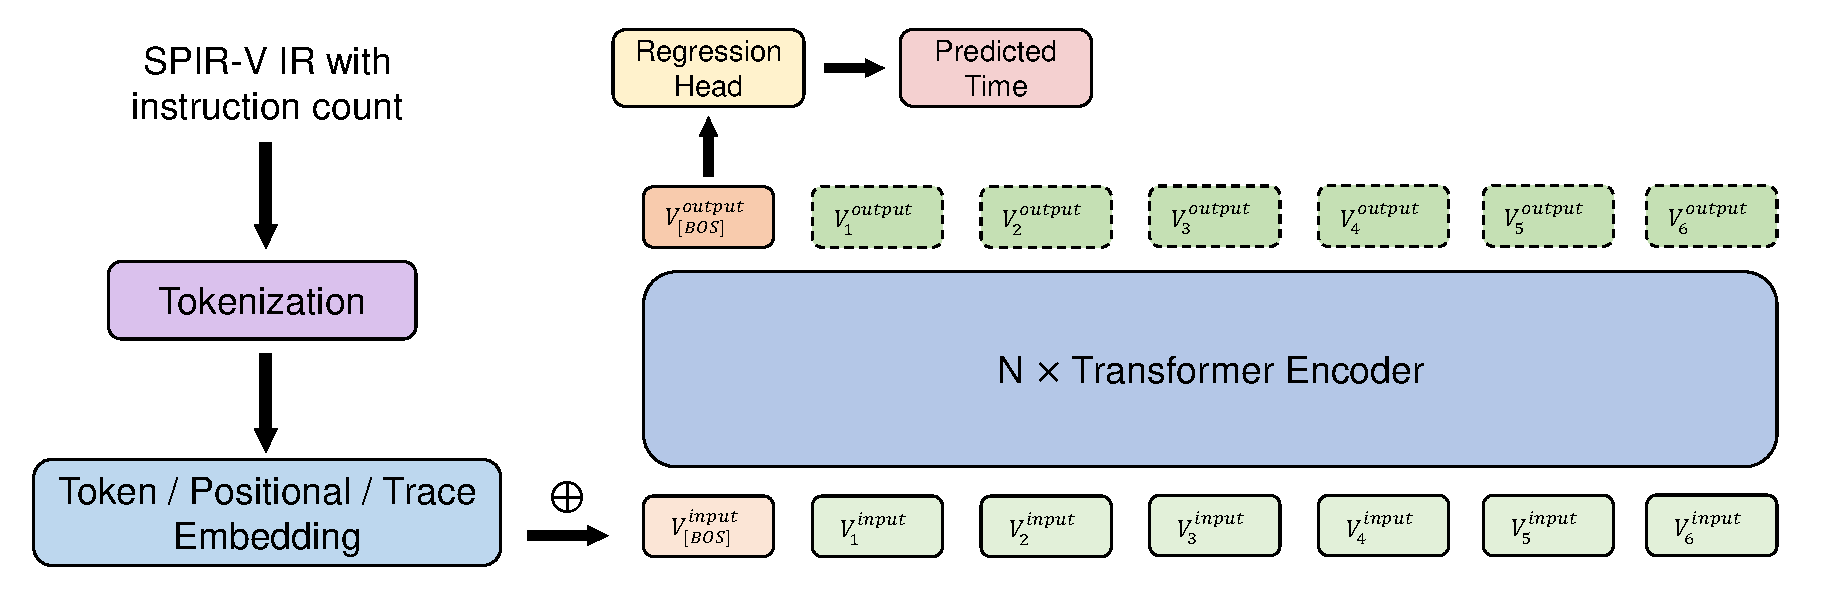
\includegraphics[width=1\linewidth]{figures/ShaderPerFormer(1)_20240103233446.pdf}
  \caption{着色器性能预测模型 ("ShaderPerFormer") 概览}
  \label{fig:spf_overview}
\end{figure}

第 \ref{sec:pl_understanding} 节提到,程序语言理解领域中广泛应用了基于 Transformer 的模型。类似的,{\amend 本章的}预测器采用类似 BERT\cite{devlin-etal-2019-bert} 架构的 Transformer 来构建回归预测模型。{\amend 为了写作方便,}下文使用该着色器程序性能模型的简称 ShaderPerFormer。

图 \ref{fig:spf_overview} 给出了 ShaderPerFormer 模型的概览。{\amend 模型的输入共分为 SPIR-V 指令和指令运行计数两个部分。SPIR-V 指令经过 SPIR-V 分词器分词后,进入嵌入生成过程。嵌入生成过程接收对应的词元和嵌入计数,并将生成的嵌入送入层叠的 Transformer 编码器,最后由回归头部取第一个词元的输出生成预测结果。下面,本节将详细介绍各个部分的设计。}

\subsubsection{SPIR-V 分词和嵌入生成}

\begin{figure}[h]
    \centering
    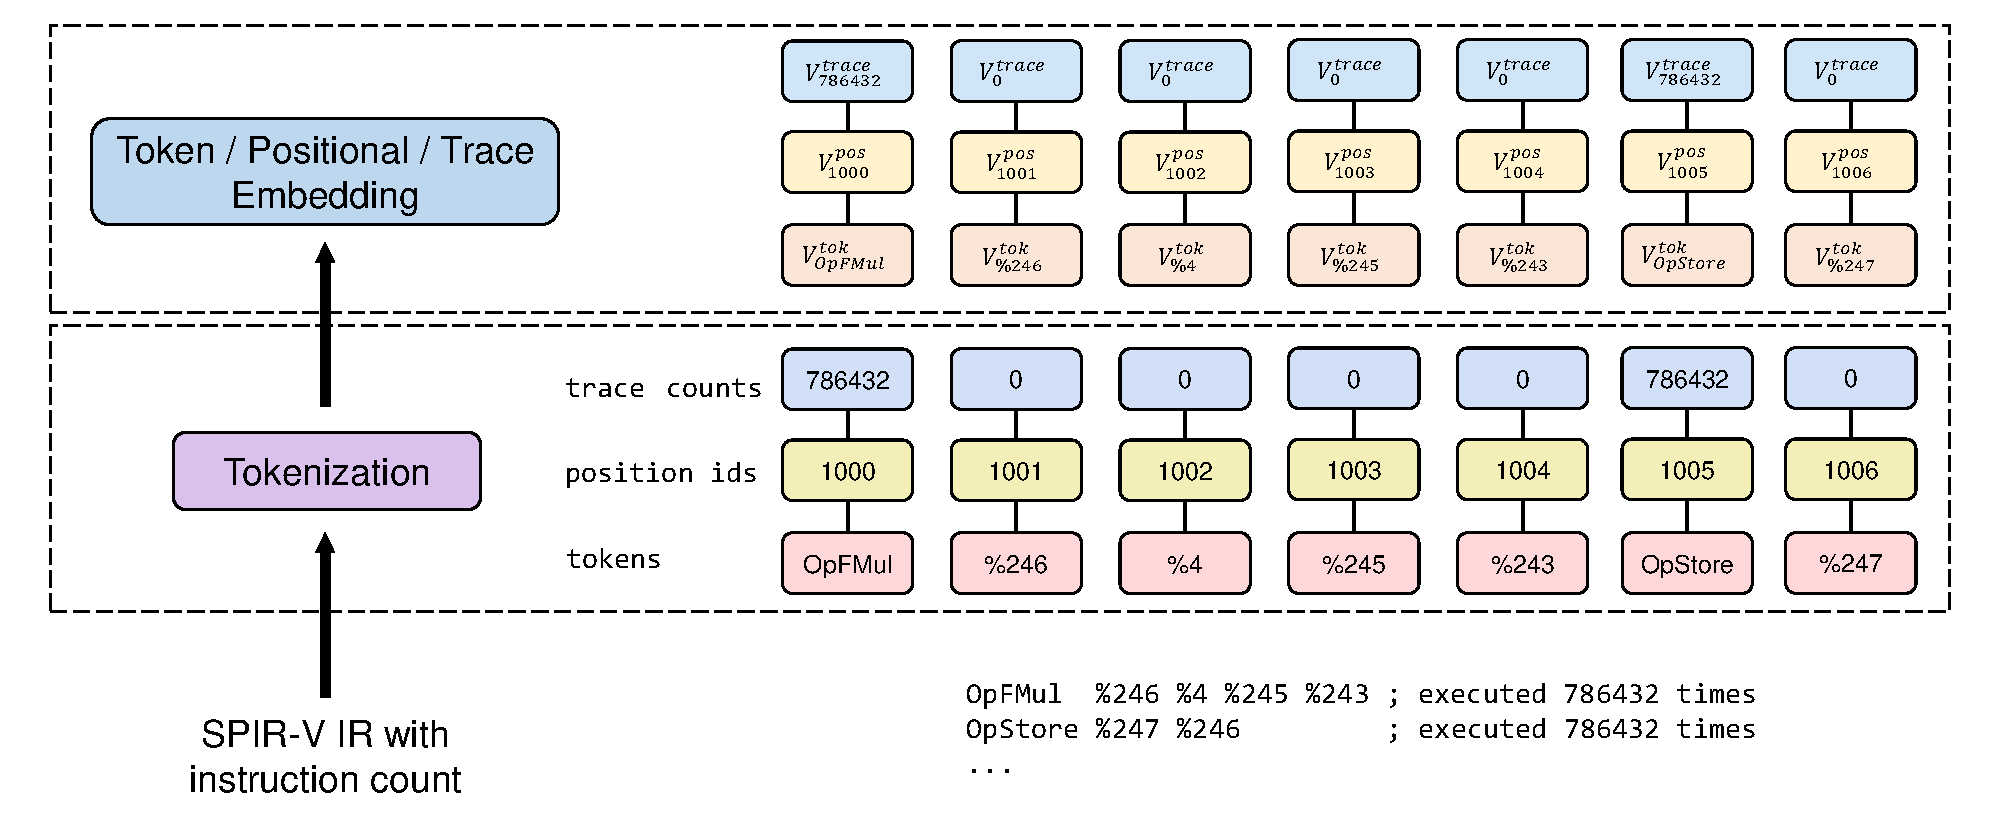
\includegraphics[width=1\linewidth]{figures/tokandembed.pdf}
    \caption{ShaderPerFormer 的分词和词嵌入向量生成过程}
    \note{注:为了可读性,分词后的操作码 (opcode) 和操作数 (operand) 词元以文本形式表示。本图展示了从位置 1000 开始的一小段中间表示指令序列,其中的指令被执行了 786432 次,正好是 1024 $\times$ 768 屏幕分辨率下每片元执行一次中间表示指令后的计数结果。因篇幅所限,OpStore 指令的操作数分词结果在此没有画出。}
    \label{fig:spf_embedding}
\end{figure}

图 \ref{fig:spf_embedding} 展示了 ShaderPerFormer 的分词和词嵌入向量生成过程。{\amend 输入 SPIR-V 指令和每条指令对应的运行计数后,首先会经由 SPIR-V 分词器按固定规则将 SPIR-V 指令转换为一到多个词元。在此之后,嵌入生成阶段会将指令的运行计数信息和指令所对应的词元对齐,进而将该条指令的运行计数生成嵌入后,与该指令的词元嵌入、位置嵌入相加,生成最终的嵌入向量。}

{\amend {\bf SPIR-V 分词}} 自然语言处理模型多使用在语料上自学习的分词器,如 BPE \cite{sennrich-etal-2016-neural}、SentencePiece \cite{kudo-richardson-2018-sentencepiece} 等。然而,由于预测模型处理的输入为 SPIR-V 指令流,故而一个{\amend 固定的分词方案}将会比基于学习的分词方案更加高效、易于编写和校验,且可以规避由于部分操作符出现次数的稀疏性给分词算法带来的问题。该方案可以实现 SPIR-V 到词元的 1:1 映射,详细算法可以参考附录中的算法 \ref{alg:tokenizer}。

{\amend {\bf 嵌入信息生成}} 指令对应的词元和其运行计数对齐后,即进入嵌入信息生成阶段。具体来说,第 $ i $ 个位置的词嵌入向量 $ \mathbf{V}^{\text{input}}_i $ 分为三个部分的组合:

\begin{equation}
\mathbf{V}^{\text{input}}_i = \mathbf{V}^\text{tok}_{t_i} +\mathbf{V}^\text{pos}_i + \mathbf{V}^\text{trace}_{m_i},
\end{equation}
其中 $t_i$ 和 $m_i$ 分别是位置 $i$ 的词元和词元对应的指令的运行计数。

$ \mathbf{V}^\text{tok}_{t_i} $ 为位置 $i$ 的词元本身的嵌入,而 $\mathbf{V}^\text{pos}_i$ 为绝对位置 $ i $ 的嵌入。和 BERT 的做法相符,这两个嵌入{\amend 均可以采用传统的、}一对一映射的可学习嵌入(learnable embedding)。$ \mathbf{V}^\text{trace}_{m_i} $ 为位置 $i$ 的词元对应的指令的运行计数的嵌入。{\amend 然而,如图 \ref{fig:bb_distrib} 所示,指令运行计数的动态范围非常大,故而需要特别实验较优秀的嵌入方式。本章的第 \ref{sec:ablation_count} 节介绍了指令计数嵌入的消融实验。}

\begin{figure}[h]
    \centering
    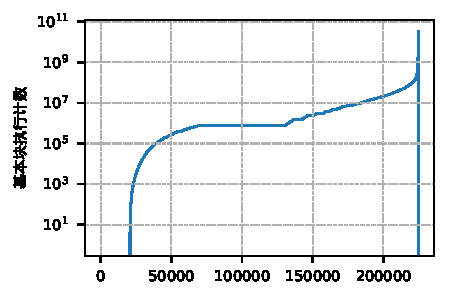
\includegraphics[width=0.6\linewidth]{figures/RTX3060_Distribution_of_basic_block_trace_count.pdf}
    \caption{着色器性能数据集中基本块执行计数的分布}
    \note{注:该图的横坐标为基本块执行计数排序后的序数,纵坐标为执行计数的值。}
    \label{fig:bb_distrib}
\end{figure}  

经过比较,本章选择了和 \citet{Born2023} 中的数值编码方案类似的方案。该方案直接将待编码的指令计数转换为二进制形式,以作为嵌入向量,并用 0 填充额外的维度。给定 $\overline{x_i}$ 表示 $x$ 的二进制表示中的第 $i$ 位数字,跟踪嵌入 $\mathbf{V}^{\text{trace}}_x$ 可以写成
\begin{equation}
\mathbf{V}^{\text{trace}}_x = [\overline{x_0}, \overline{x_1}, \dots, \overline{x_{63}}, 0, \dots, 0].
\end{equation}

值得注意的是,SPIR-V 中的一个指令经常有多个操作数,而其每个操作数根据算法 \ref{alg:tokenizer} 又可能对应多个词元。在所有这些词元的指令计数嵌入中,只有第一个词元的指令计数嵌入 $ \mathbf{V}^{\text{trace}} $ 会可能被设置为非零向量。

\subsubsection{编码器输出、归一化和损失函数}

{\amend {\bf 编码器和输出层}} 模型的骨干网络使用 9 层的 Transformer 编码器,隐藏层维度为 768,注意力头数为 12。最后一层的 Transformer 编码器后连接着输出层。输出层会选取第一个词元(固定为 \verb|[BOS]|)对应的特征向量,并将其送入回归头进行输出预测。选择固定的 \verb|[BOS]| 词元对应的特征向量的主要原因是为了增强模型的稳定性。Transformer 模型的每一层都会在所有词元位置处计算注意力,而一个稳定的固定词元作为输出可以降低不稳定的后续输入对输出带来的影响。此种做法在 BERT \cite{devlin-etal-2019-bert}中也得到了应用。

{\amend 回归头同样采用常规设计,}其计算方式如下:
\begin{equation}
    \label{eq:reg_head}
    \text{RegressionHead}(x) = \text{Linear}(\text{Dropout}(\text{Tanh}(\text{Linear}(\text{Dropout}(x))))).
\end{equation}

{\amend {\bf 归一化} 着色器性能样本在时间特征上的分布在第 \ref{sec:shader_performance_data} 节中的图 \ref{fig:archTimeMean_ch3} 中已有所展示。从中可以看到,}性能样本时间跨度从 $10^{-6}$ 秒到 $10^{-1}$ 秒不等。{\amend 前期实验表明,只有相对正确的归一化方法才可以使得模型达到可用的性能表现。第 \ref{sec:ablation_normalize} 节中给出了归一化与损失函数的探索。}

{\amend 经过实验,}本章最终选择使用对数函数对着色器性能样本进行归一化,即对数据集中的每一个时间 $t$ 都进行 $\log(t)$ 变换,同时使用均方误差(MSE)作为 ShaderPerFormer 的损失函数。考虑到使用的归一化方法,该损失函数也可以被称为均方对数误差(Mean Squared Logarithmic Error,MSLE)。在对数尺度上,数据的变化更加平滑,这有助于模型更好地学习数据的分布。同时,MSLE 损失函数鼓励模型对预测值和真实值的对数进行准确的估计,从而在指数变换回原始尺度后,能够获得较为准确的预测结果。

\section{{\amend 实验和分析}}

% 同时,由于 ShaderPerFormer 需要将整个着色器程序的 SPIR-V 作为模型的输入,这样一来,模型可以接受的序列长度将直接影响其训练和使用时的泛用性。针对于 Transformer 训练时内存占用较高的问题,我们在 Transformer 的编码器中的注意力部分使用了低内存占用的 Memory Efficient Attention \cite{rabe2022selfattention} 注意力实现。

{\amend 本节将给出证明本章提出的着色器程序性能预测方法的有效性的实验,以及其各个部分设计决策的相关支撑实验。本章首先会给出现有基线模型的相关讨论,然后给出本章方法和基线方法在着色器性能数据集和其挑战样本集上的性能表现,最后再给出三个消融和对比实验。}

\subsection{基线模型}

{\amend 第 \ref{sec:ch4_intro} 节引言的讨论中提到,着色器性能预测模型在学术界并没有得到充分的挖掘,一系列着色器优化工作都使用直接测量或者简单线性模型的方式对着色器性能进行评估。着色器性能优化工作的最先进实现仍然依赖 \citet{10.1145/2816795.2818104} 的工作提出的启发式。}该启发式采用下式来估计着色器在一个绘制流水线阶段的性能,
\begin{align}
t &= N_\text{scalarOps} + 100 \times N_\text{textureOps},
\end{align}
其中 $N_\text{scalarOps}$ 是着色器程序中标量操作的数目, $N_\text{textureOps}$ 是着色器程序中纹理采样操作的数目。这里的常数 $100$ 是一个原方法中随意设置的值,用于表示标量操作和浮点操作之间性能的相对关系。

将这个思路进行简单的推广后,{\amend 本节}使用两种方法来作为基线,
\begin{align}
\label{eq:sh} t &= c_\text{inst} \cdot N_\text{inst} \\
\label{eq:pilr} t &= \sum_{i=1}^{M} c_{\text{inst}_{i}} \cdot N_{\text{inst}_{i}}.
\end{align}

\begin{enumerate}
    \item 简单启发式(Simple Heuristics,SH): 如式 (\ref{eq:sh}),IR 中的每条指令都赋予一个统一的指令时间开销 $c_{inst}$,并且乘以着色器运行时执行总 IR 指令数 $N_{inst}$,以得到预测的着色器运行总时间。
    \item 逐指令线性回归(Per Instruction Linear Regression,PILR): 如式 (\ref{eq:pilr}) 所示,IR 中的每种指令赋予一个统一的时间开销 $c_{inst_i}$,并且乘以该种指令运行时执行的总次数 $N_{inst_i}$,并对每个指令种类求和,以得到预测的着色器运行总时间。
\end{enumerate}

{\amend 体系结构模拟器中,如 Emerald\cite{10.1145/3307650.3322221},实现了图形系统的建模。然而,在前期实验中发现,该模拟器对着色器的执行,使用 Mesa 的 TGSI \cite{TGSI} 翻译到 CUDA 的 PTX 指令,进而送入 GPGPU-Sim 完成对应的 SIMD 核心模拟。TGSI 到 PTX 的翻译过程中,Emerald 并没有处理循环指令,使得绝大多数 Shadertoy 着色器都无法运行。此外,Emerald 需要进行细致的参数调节,使得模拟的架构和真实的架构基本相似。原论文中,Emerald 通过调节参数模拟 Tegra K1 SoC 的运行过程中,在 14 个测试程序上实现了从 5.2\% 到 312\%,平均 32.2\% 的相对预测误差表现。考虑到比较上的难度和意义,本节没有将 Emerald 加入比较。}

\subsection{数据集划分和训练}
\label{sec:split_and_training}

{\amend 着色器数据集工作中的}图 \ref{table:datasetFilters_ch3} 给出了经过过滤后的各个架构中的着色器性能样本。每个性能样本都对应着一个着色器,而鉴于各个平台上被过滤后剩下的性能样本数量不一,如果将每个平台剩余的性能样本单独进行数据集划分的话,则可能因为在不同平台上不一致的划分影响后续评估的有效性。故而,{\amend 本节}首先将不同平台剩余的性能样本对应的着色器取并集,在这个并集中将性能样本随机划分为训练集、测试集和验证集,且比例为训练集:测试集:验证集=$80:5:15$。

模型的训练使用一块 24 GB 显存的 NVIDIA GeForce RTX 4090 完成。得益于 xformers \cite{xFormers2022}库中 Memory Efficient Attention 的注意力算子实现\cite{rabe2022selfattention},{\amend 本章提出的}模型可以在第 \ref{sec:model_construction} 节提及的模型配置下使用 4096 的最大序列长度进行训练。在上述模型配置下,{\amend 本节}使用 2 的批次大小(batchsize),并通过 20 步的梯度累积(gradient accumulation)来得到 40 的等效批次大小。

{\amend 本节}使用 Adam \cite{Kingma2014AdamAM} 作为优化器,学习率设为 $3 \times 10^{-5}$,使用默认的 Adam 配置($\beta_1=0.9, \beta_2=0.999, \epsilon=1 \times 10^{-8}$),并使用预热比例(warmup ratio)为 0.1 的线性学习率预热。每种架构上的模型均训练 50 个迭代轮次(epoch),并挑选出在轮次结束时,在测试集上具有最佳 MAPE (Mean Average Percentage Error, 平均绝对百分比误差)的模型权重作为最优模型权重,并作为后续评估使用的模型。

\subsection{基线比较}

{\amend 本节}在收集的 5 个平台上分别评估了两种基线方法和本文所述预测模型的性能,并在划分出的验证集上报告预测时间与实际测量时间之间的 MAPE。评估的结果参见表 \ref{table:mainResults}。

从表中可以看出,本章提出的方法在所有测试方法中是最准确的。与简单启发式方法和逐指令线性回归这两种基线方法相比,{\amend 本章}提出的方法在 5 个待测平台上的平均 MAPE 分别提高了 25.25\% 和 8.26\%,并达到了 35.96\% 的平均 MAPE。

对于着色器优化任务来说,在进行优化变体评估时通常只需要确定给定的变体之间的性能的相对排序,而不需要其绝对值。这种情形下的准确度可以用 Spearman 相关系数来进行刻画。Spearman 相关系数可以刻画两个统计变量之间的秩的相关性,且当两组统计观测值之间由相似的秩时相关系数较高。两组组在秩的意义下完美单调增加的序列的 Spearman 相关系数为 1。表 \ref{table:mainResults} 还同时报告了每种方法的预测结果与测量结果之间的 Spearman 相关系数。与其它基线方法相比,{\amend 本章提出的}方法在所有测试平台上都拥有最高的 Spearman 相关系数。

MAPE 和 Spearman 系数缺乏对于不同运行时间分组的着色器性能样本,其预测精度的刻画能力。如图 \ref{fig:archHeatmap} 所示,为了让三种预测模型的结果得到更直观的展示,{\amend 本章}给出了在各个平台上,基线模型和{\amend 本章提出的}方法的预测和实际结果的分布热力图。该热力图的横轴为测量得到的 10 次真实时间的均值,纵轴为性能预测模型预测的时间。热力图的中央部分被切分为 50 $\times$ 50 的格子,每个格子中用颜色表示该区域中分布的样本数量。可以看出,{\amend 本章提出的}模型较其它两个模型,在较高性能和较低时间的性能样本部分都拥有不错的表现,且接近 $y=x$ 的直线。

\begin{figure}[htbp]
  \centering
  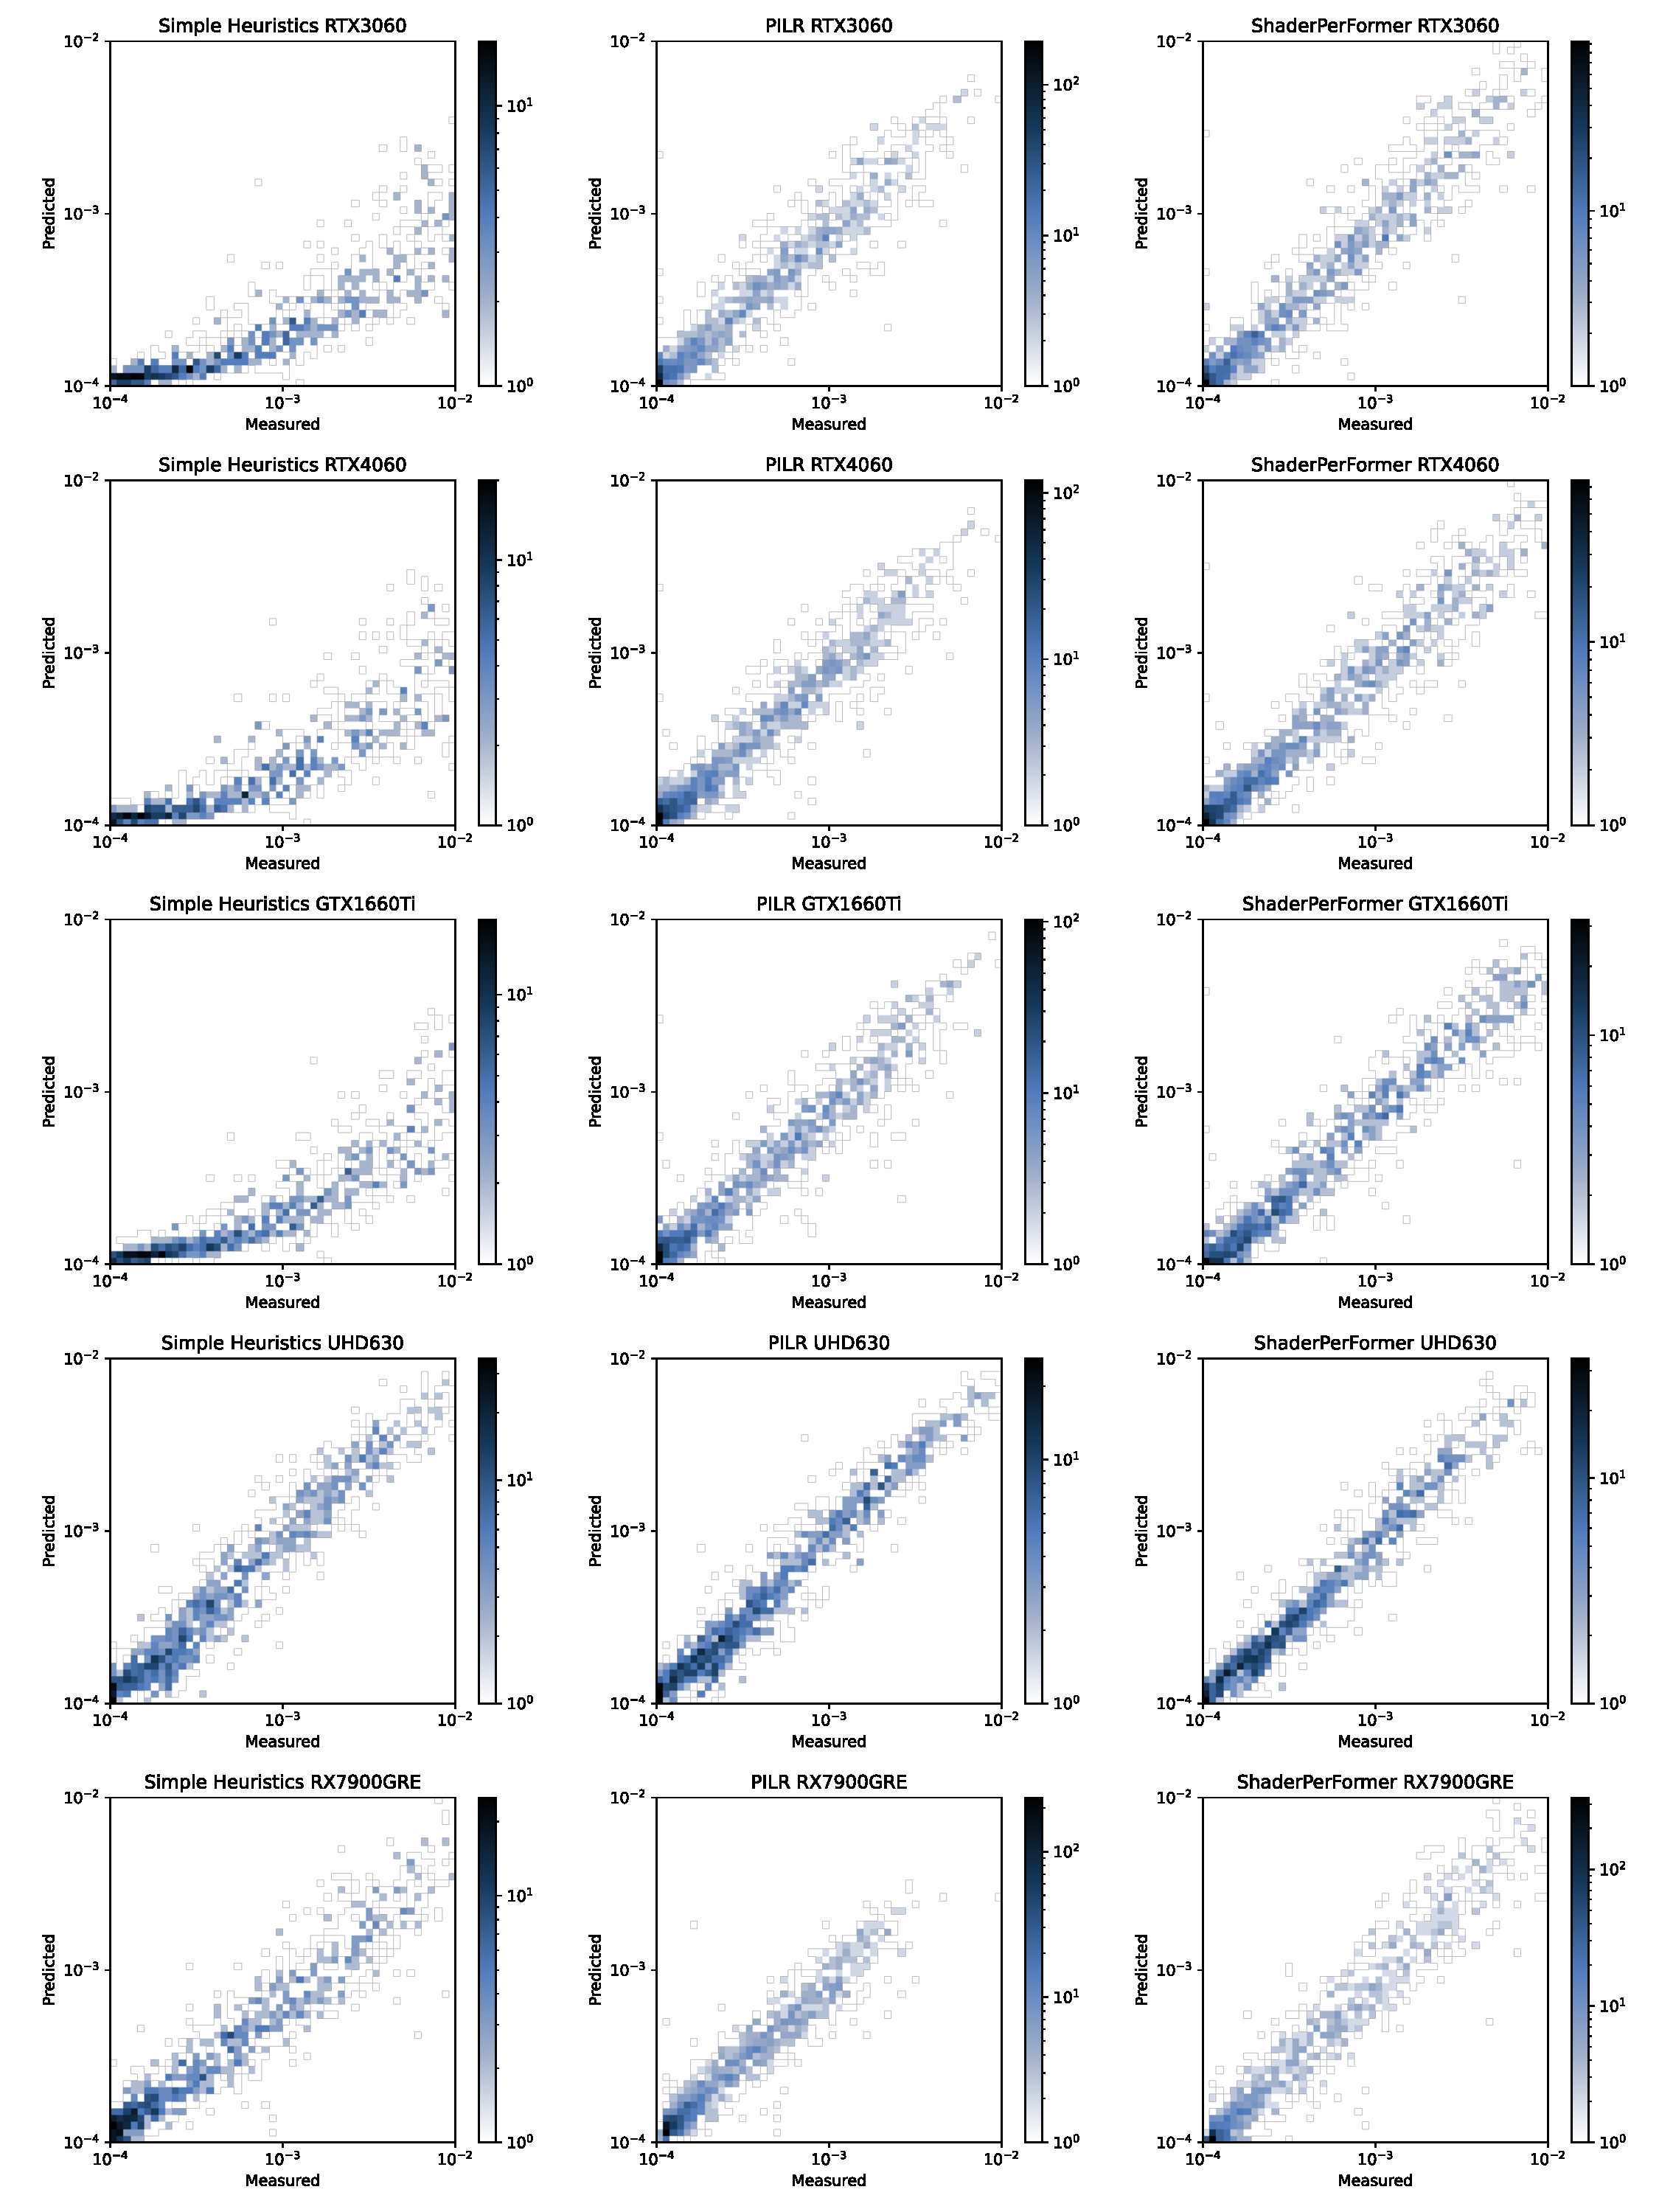
\includegraphics[width=1.0\linewidth]{figures/archHeatmapRefined.pdf}
  \caption{各个平台上,基线模型和本文方法的预测和实际结果的分布热力图}
  \note{注:SH 代表简单启发式,PILR 代表逐指令线性回归,ShaderPerFormer 代表本研究提出的基于神经网络的着色器性能预测方法。}
  \label{fig:archHeatmap}
\end{figure}

这些评估结果表明,{\amend 本章提出的方法}在预测着色器性能方面相比于基线方法具有一定比较优势,特别是在需要对多个着色器进行性能排序的场景中。Spearman 相关系数的高值表明,{\amend 本章提出的方法}能够更有效地进行着色器性能排序,这对于开发者进行着色器性能优化有一定价值。此外,{\amend 本章提出的方法}在需要精确性能评估的场合,较现有的着色器性能评估工作也更具有竞争力。

\begin{table}[h]
    \centering
    \caption{各 GPU 平台上的验证集下的模型性能结果}
    \label{table:mainResults}
    \begin{tabular}{l|cccccc}
    \toprule
    % \multicolumn{3}{c}{\textbf{MAPE}}
    % \multirow{2}{*}{\textbf{Platform}}
        ~  & \multicolumn{2}{c}{SH} & \multicolumn{2}{c}{PILR} & \multicolumn{2}{c}{ShaderPerFormer (\textbf{Ours})} \\ 
        \textbf{平台}          & MAPE & Spearman & MAPE & Spearman & MAPE & Spearman \\
    \midrule
        RTX3060 &  75.26\% & 0.9584 &  46.90\% & 0.9200 & \textbf{40.44\%} & \textbf{0.9642} \\
        UHD630 &  30.73\% & 0.9594 &  27.32\% & 0.9676 & \textbf{26.60\%} & \textbf{0.9722} \\
        RTX4060 &  81.17\% & 0.9588 &  55.60\% & 0.9290 & \textbf{44.62\%} & \textbf{0.9632} \\
        GTX1660Ti &  82.56\% & 0.9607 &  54.99\% & 0.9353 & \textbf{41.59\%} & \textbf{0.9681} \\
        RX7900GRE &  36.32\% & 0.9510 &  36.28\% & 0.9433 & \textbf{26.54\%} & \textbf{0.9578} \\
    \midrule
        平均 & 61.21\% & --- & 44.22\% & --- & \textbf{35.96\%} & --- \\
    \bottomrule
    \end{tabular}
    \note{注:SH 代表简单启发式,PILR 代表逐指令线性回归,ShaderPerFormer 代表本章提出的数据驱动的着色器性能预测方法。最佳的性能指标以加粗字体展示。}
\end{table}

\subsection{{\added 挑战样本集基线比较}}

{\added 第 \ref{sec:challenge_set_construction} 节给出了着色器性能挑战样本集的构造过程,该集合中的着色器在不同平台上的性能差异较其它着色器明显。故而,本节将给出挑战样本集上本章提出的方法和基线方法的性能比较。}

\begin{table}[h]
    \centering
    \caption{各 GPU 平台上的挑战样本集下的预测结果}
    \label{table:challengeResults}
    \begin{tabular}{l|cccccc}
    \toprule
          ~   & \multicolumn{2}{c}{SH} & \multicolumn{2}{c}{PILR} & \multicolumn{2}{c}{ShaderPerFormer (\textbf{Ours})} \\
    平台       & MAPE       & Spearman    & MAPE       & Spearman    & MAPE            & Spearman          \\
    \midrule
    RTX3060   & 74.94\%     & 0.9621      & 35.24\%     & 0.9107      & \textbf{32.08\%}  & \textbf{0.9690}  \\
    RTX4060   & 80.94\%     & 0.9535      & 42.00\%     & 0.8993      & \textbf{34.02\%}  & \textbf{0.9579}  \\
    UHD630    & 30.93\%     & 0.9582      & 29.83\%     & 0.9621      & \textbf{27.30\%}  & \textbf{0.9685}  \\
    GTX1660Ti & 80.20\%     & 0.9590      & 40.34\%     & 0.9306      & \textbf{37.06\%}  & \textbf{0.9676}  \\
    RX7900GRE & 37.69\%     & 0.9445      & 27.38\%     & 0.9347      & \textbf{27.07\%}  & \textbf{0.9535}  \\
    \midrule
    平均       & 60.94\% & --- & 34.96\% & --- & \textbf{31.51\%} & --- \\
    \bottomrule
    \end{tabular}
    \note{注:SH 代表简单启发式,PILR 代表逐指令线性回归,ShaderPerFormer 代表本章提出的数据驱动的着色器性能预测方法。最佳的性能指标以加粗字体展示。}
\end{table}

{\added 从表 \ref{table:challengeResults} 中可以看出,在挑战数据集下本章提出的方法仍然表现良好,且优于其它两个基线方法。}

\subsection{指令计数信息}
\label{sec:ablation_trace}

{\amend 第 \ref{sec:design_decisions} 节中提到,指令计数信息对于预测模型的表现有重要影响。}为了证明{\amend 本文}提出的指令计数信息对着色器性能预测任务的重要性,本节对比在没有指令计数信息的的情况下,{\amend 本章提出的}方法和基线方法的性能。

为了确保公平比较,在消融实验中{\amend 本节}保持模型的网络架构不变,并将所有位置的指令计数设置为 1。这意味着所有位置的指令计数嵌入均变为了 $\mathbf{V}^\text{trace}_{1} = [1, 0, \dots, 0]$,从而消除了指令的追踪信息产生的计数的嵌入对网络的影响。

对于简单启发式和逐指令线性回归两种基线方法,{\amend 本节}进行如下的更改:
\begin{enumerate}
    \item 简单启发式:将式 (\ref{eq:sh}) 中的 $N_{inst}$ 由着色器\textbf{运行时}执行的总 IR 指令数替换为着色器程序总 IR 指令数
    \item 逐指令线性回归:将式 (\ref{eq:pilr}) 中的 $N_{inst_i}$ 由着色器\textbf{运行时}执行的该种指令数目替换为着色器该种指令数目
\end{enumerate}

对于基线方法的修改相当于,在两种基线方法训练时,假设着色器中的每条指令“执行”一次且仅“执行”一次,其余细节保持不变。

如表 \ref{table:ablationTrace} 所示,指令跟踪被证明对于 ShaderPerFormer 和逐指令线性回归方法起到了在 MAPE 和 Spearman 相关系数意义上、对不同待测 GPU 平台一致的效果改善,在简单启发式模型中,部分平台的 MAPE 测量结果得到了效果改善,而所有平台的 Spearman 相关系数都得到了改善。

这一结果证明了指令计数信息对着色器性能预测任务的重要性。通过考虑指令的实际执行次数,{\amend 本章的}方法能够更准确地预测着色器的执行时间。这种改进对于ShaderPerFormer 和 PILR 这样{\amend 的}模型尤其重要,因为它们依赖于输入数据的质量和代表性来做出准确的预测。简单启发式方法虽然在某些平台上表现出了改进,但可能不如前两者那样一致或显著,这也表明更复杂的模型可以更好地利用指令计数信息。

\begin{table}[h]
    \centering
    \caption{在 ShaderPerFormer 和两种基线方法上进行的指令追踪信息的消融实验结果}
    \label{table:ablationTrace}
    \begin{tabular}{l|l|cccc}
    \toprule
        \multirow{2}{*}{\textbf{方法}} & \multirow{2}{*}{\textbf{平台}} & \multicolumn{2}{c}{\textbf{MAPE}} & \multicolumn{2}{c}{\textbf{Spearman}} \\ 
        ~                                & ~                                  & 无追踪信息 & 有追踪信息 & 无追踪信息 & 有追踪信息 \\ 
    \midrule
        \multirow{5}{*}{SH}   & RTX3060             & 76.02\%  & \textbf{75.26\%} &  0.7131 &  \textbf{0.9584} \\
        ~ & UHD630                                  & 66.97\%  & \textbf{30.73\%} &  0.7152 &  \textbf{0.9594} \\
        ~ & RTX4060                                 & \textbf{79.54\%}  & 81.17\% &  0.7118 &  \textbf{0.9588} \\
        ~ & GTX1660Ti                               & \textbf{80.20\%}  & 82.56\% &  0.7142 &  \textbf{0.9607} \\
        ~ & RX7900GRE                               & 68.65\%  & \textbf{36.32\%} &  0.6857 &  \textbf{0.9510} \\ \hline
        \multirow{5}{*}{PILR} & RTX3060             & 86.43\%  & \textbf{46.90\%} &  0.8551 &  \textbf{0.9200} \\
        ~ & UHD630                                  & 72.87\%  & \textbf{27.32\%} &  0.8503 &  \textbf{0.9676} \\
        ~ & RTX4060                                 & 90.39\%  & \textbf{55.60\%} &  0.8563 &  \textbf{0.9290} \\
        ~ & GTX1660Ti                               & 90.26\%  & \textbf{54.99\%} &  0.8571 &  \textbf{0.9353} \\
        ~ & RX7900GRE                               & 81.19\%  & \textbf{36.28\%} &  0.8388 &  \textbf{0.9433} \\ \hline
        \multirow{5}{*}{\makecell{ShaderPerFormer \\(\textbf{Ours})}} & RTX3060              & 81.02\%  & \textbf{40.44\%} &  0.8608 &  \textbf{0.9642} \\
        ~ & UHD630                                  & 70.42\%  & \textbf{26.60\%} &  0.8749 &  \textbf{0.9722} \\
        ~ & RTX4060                                 & 98.10\%  & \textbf{44.62\%} &  0.7518 &  \textbf{0.9632} \\
        ~ & GTX1660Ti                               & 109.60\% & \textbf{41.59\%} &  0.8784 &  \textbf{0.9681} \\
        ~ & RX7900GRE                               & 51.16\%  & \textbf{26.54\%} &  0.8448 &  \textbf{0.9578} \\
    \bottomrule
    \end{tabular}
    \note{注:SH 代表简单启发式,PILR 代表逐指令线性回归,ShaderPerFormer 代表本章提出的基于数据驱动的着色器性能预测方法。最佳的性能指标以加粗字体展示。}
\end{table}

\subsection{{\added 指令计数嵌入的构造方式}}
\label{sec:ablation_count}

{\added 本节实验了不同的指令计数嵌入构造方式对于着色器性能预测模型表现的影响。下面将分别介绍实验的嵌入方法。

{\bf 直接压缩}方法会直接将每个指令对应的指令计数除以可能取到的最大指令计数,然后作为该指令的指令计数嵌入。如图 \ref{fig:bb_distrib} 所示,在用于测试的着色器性能数据集中,最大的指令计数为 $ 3.68 \times 10^{10} $,故而此处选择保守的除以 $ 5 \times 10^{10} $。

{\bf logPlus 变换}方法会将计数 $ c_i $ 使用 logPlus 变换,即将 $ \log(c_i + 1) $ 作为对应位置的指令计数嵌入。

{\bf 二进制嵌入}即本章构造的模型使用的方法。该方法的思想来源于 \citet{Born2023} 的工作,但更为简单。该方法的主要步骤为,将指令计数嵌入值 $ x $ 按二进制位展开后的结果送入网络,同时在高位补充 0 作为填充。

{\bf 二进制可学习嵌入}方法的思想来源于 \citet{DBLP:journals/corr/abs-2106-11959} 关于表格数据处理中数字特征编码的工作。该方法和二进制嵌入方法的差异在于,其在获得二进制嵌入向量 $ x $ 后,设 $ x $ 共有 $ m $ 个二进制位,则进一步的对 $ x $ 每个二进制位,针对其 0 或 1 的状态进行查表,得到 $ m $ 个可学习的嵌入,再将这些嵌入加和。每个 0 或者 1 都有一个独特的可学习嵌入,故总的可学习嵌入数量为 $ 2m $,每个可学习嵌入的维度都和隐藏层维度相同。

{\bf 二进制可学习嵌入 + 截断}则是观察到了二进制可学习嵌入的一个缺陷,即表示较大数字的二进制位,其非零值出现概率较小,则其嵌入被训练的次数较少。这样一来,在遇到极端值时,二进制可学习嵌入的表现反而可能变差。截断处理会将大于 $ 2^k $ 的指令计数截断为其所能表示的最大值 $ 2^k $,而不管其是否更大。根据最高的几个二进制位出现的频率分析,此处取 $ k = 30 $。

表 \ref{table:ablationTraceEmbed} 给出了上面设计的五种方法对模型表现的影响,其中最佳指标以加粗字体展示。为了节约时间,此处实验设置的训练轮次为 20 轮,其余设置与第 \ref{sec:split_and_training} 节给出的训练细节相符。

从表中可以看出,本章使用的二进制嵌入方法表现最佳。直接压缩和 logPlus 变换法均大幅落后于该方法,二进制可学习嵌入在加入截断的情况下表现有所提升,但仍稍稍落后于本章使用的方法。
}

\begin{table}[h]
    \centering
    \caption{指令计数嵌入的构造方式对于模型表现的影响}
    \label{table:ablationTraceEmbed}
    \resizebox{\textwidth}{!}{%
    \begin{tabular}{l|ccccc}
        \toprule
        ~ & 直接压缩     & logPlus 变换 & 二进制嵌入            & 二进制可学习嵌入 & 二进制可学习嵌入 + 截断    \\
        \midrule
        平台        & MAPE     & MAPE       & MAPE             & MAPE     & MAPE             \\
        \midrule
        RTX3060   & 86.14\%  & 57.82\%    & \textbf{37.14\%} & 40.02\%  & 40.50\%          \\
        RTX4060   & 71.96\%  & 58.24\%    & \textbf{39.64\%} & 41.49\%  & 43.80\%          \\
        UHD630    & 91.65\%  & 66.42\%    & \textbf{27.65\%} & 29.04\%  & 28.23\%          \\
        GTX1660Ti & 109.34\% & 63.33\%    & 43.02\%          & 47.11\%  & \textbf{42.84\%} \\
        RX7900GRE & 50.18\%  & 52.30\%    & \textbf{27.73\%} & 27.99\%  & 29.08\%          \\
        \midrule
        平均      & 81.85\%  & 59.62\%    & \textbf{35.04\%} & 37.13\%  & 36.89\% \\
        \midrule
        ~         & Spearman & Spearman   & Spearman         & Spearman & Spearman         \\
        \midrule
        RTX3060   & 0.8786   & 0.8071     & \textbf{0.9660}  & 0.9400   & 0.9536           \\
        RTX4060   & 0.8787   & 0.7521     & \textbf{0.9669}  & 0.9658   & 0.9666           \\
        UHD630    & 0.8654   & 0.7707     & \textbf{0.9716}  & 0.9685   & 0.9694           \\
        GTX1660Ti & 0.8658   & 0.8125     & \textbf{0.9693}  & 0.9650   & 0.9676           \\
        RX7900GRE & 0.8634   & 0.8220     & 0.9576           & 0.9555   & \textbf{0.9585}  \\
        \bottomrule
    \end{tabular}%
    }
\end{table}

\subsection{{\added 性能样本时间归一化和损失函数设计}}
\label{sec:ablation_normalize}

{\added 第 \ref{sec:model_construction} 节提到,预测模型的设计过程中,性能样本的时间所使用的归一化方式和损失函数的设计对于模型表现均有一定影响。第 \ref{sec:shader_performance_data} 节的图 \ref{fig:archTimeMean_ch3} 给出了性能样本的时间分布特征,而本节则实验了不同时间归一化方式和损失函数的设计对于模型表现的影响。下面将分别介绍实验组。

{\bf 无归一化 + MSE}组给出了不进行归一化的模型性能。由于模型本身的正则化方法以及训练时优化器的设置,无归一化的训练的结果处于不可用状态。

{\bf 样本归一化 + MSE}组给出了使用标准的均值-标准差归一化技术来进行归一化后的模型表现。该归一化方法首先会统计训练样本性能的均值和方差,以便将数据分布通过线性变换调整至均值为 0,标准差为 1 的状态,然后再进行训练。可以看到,其效果仍然不甚理想。

{\bf log + MSE}组使用了本章所构造的模型使用的归一化和损失函数。该组的表现最为出色。{\bf logPlus + MSE}组则是采用 $ \log(t+1) $ 的对数变换,而非 $ \log(t) $ 的对数变换来变换时间样本。可以看到,该组的表现并不理想。

{\bf 无归一化 + MAPE}组使用了 MAPE 作为损失函数进行优化。使用 MAPE 的原因为,着色器指令执行的相对预测误差较绝对预测误差更有意义,因为着色器的运行时间可以看成一系列指令运行的时间之和,若将每个指令的执行时间建模为独立同分布的、均值为 $ \mu $,标准差为 $ \sigma $ 的随机变量,则若干指令的执行时间的和的分布的方差和均值之比为常数。故而,MAPE 作为相对误差,其规模是不随程序规模变化而变化的。然而,MAPE 并不能应用在其它归一化后的时间中,因为 MAPE 损失函数使用了比值,而比值需要目标值和预测值都有正确的零点。本组探索了单独使用 MAPE 的有效性。可以看到,单独使用 MAPE 进行优化的效果并不好。

\begin{figure}[htbp]
    \centering
    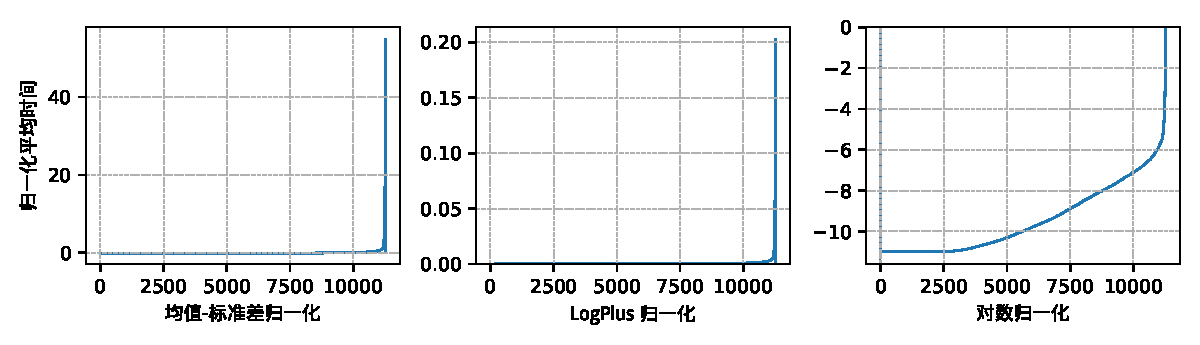
\includegraphics[width=1.0\linewidth]{figures/RTX3060-Mean-Time-Normalized.pdf}
    \caption{样本归一化、logPlus 和 log 归一化后的时间样本分布统计}
    \label{fig:normalize_methods}
\end{figure}

图 \ref{fig:normalize_methods} 给出了样本归一化、logPlus 和 log 归一化后的时间样本分布统计。从该图中可以看到,只有 log 归一化后数据分布较为均匀。这可以作为 log 归一化对本模型表现提升的解释。

}

\begin{table}[h]
    \centering
    \caption{性能样本时间归一化和损失函数设计对于模型表现的影响}
    \label{table:ablationNormalization}
    \resizebox{\textwidth}{!}{%
\begin{tabular}{l|ccccc}
\toprule
          & 无归一化 + MSE & 样本归一化 + MSE & log + MSE        & logPlus + MSE & 无归一化 + MAPE \\
\midrule
平台        & MAPE       & MAPE        & MAPE             & MAPE          & MAPE        \\
\midrule
RTX3060   & 4950.69\%  & 124.96\%    & \textbf{37.14\%} & 913.74\%      & 178.86\%    \\
RTX4060   & 2658.23\%  & 115.72\%    & \textbf{39.64\%} & 1533.74\%     & 147.57\%    \\
UHD630    & 404.76\%   & 41.26\%     & \textbf{27.65\%} & 699.16\%      & 330.78\%    \\
GTX1660Ti & 1073.23\%  & 134.64\%    & \textbf{43.02\%} & 3069.44\%     & 863.09\%    \\
RX7900GRE & 456.03\%   & 106.62\%    & \textbf{27.73\%} & 612.91\%      & 285.05\%    \\
平均        & 1908.59\%  & 104.64\%    & \textbf{35.04\%} & 1365.80\%     & 361.07\%    \\
        \midrule
          & Spearman   & Spearman    & Spearman         & Spearman      & Spearman    \\
          \midrule
RTX3060   & 0.6801     & 0.8586      & \textbf{0.9660}  & 0.7368        & 0.5098      \\
RTX4060   & 0.7085     & 0.8853      & \textbf{0.9669}  & 0.7557        & 0.3294      \\
UHD630    & 0.8378     & 0.9418      & \textbf{0.9716}  & 0.7904        & 0.5490      \\
GTX1660Ti & 0.7629     & 0.9124      & \textbf{0.9693}  & 0.6963        & 0.1756      \\
RX7900GRE & 0.6662     & 0.8517      & \textbf{0.9576}  & 0.4148        & 0.3631      \\
\bottomrule
\end{tabular}%
}
\end{table}

\section{{\added 本章小结}}

{\added 本章提出了数据驱动的着色器程序性能预测方法。本章在引言部分,提出了着色器程序性能预测面临的诸多挑战,并在之后一节系统阐述了本章提出方法的针对性的设计思路。然后,本章详细介绍了该着色器程序性能预测方法的实现,包括指令计数跟踪和模型构建两个大任务下的诸多细节和子模块。在这之后,本章给出了基线方法和相关讨论,并分别给出了基线比较、挑战样本集基线比较、指令计数信息的消融实验、指令计数嵌入的对比试验,以及性能样本时间归一化和损失函数设计的相关实验。}